\documentclass[tikz]{standalone}
\usetikzlibrary{automata, positioning}

\begin{document}
	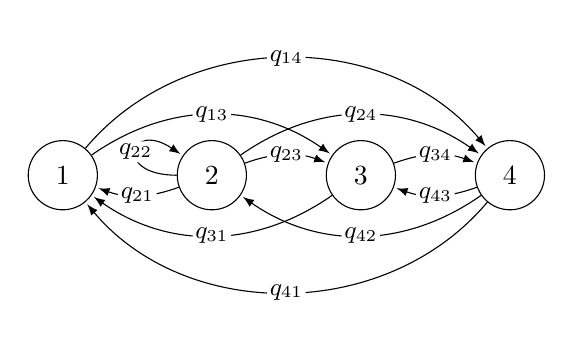
\begin{tikzpicture}
	\tikzset{
		in place/.style={
			auto=false,
			fill=white,
			font=\small,
			inner sep=1pt,
            rounded corners=1pt
		},
	}

	\node[state] (1) {1};
	\node[state, right=of 1] (2) {2};
	\node[state, right=of 2] (3) {3};
	\node[state, right=of 3] (4) {4};
	
	\draw[
	>=latex,
	auto=right,
	every loop,
	]
	(1) edge[bend left=35] node[in place] {$q_{13}$} (3)
	(1) edge[bend left=50] node[in place] {$q_{14}$} (4)
	(2) edge[bend left=20] node[in place] {$q_{21}$} (1)
	(2) edge[out=180, in=146, loop] node[in place] {$q_{22}$} (2)
	(2) edge[bend left=20] node[in place] {$q_{23}$} (3)
	(2) edge[bend left=35] node[in place] {$q_{24}$} (4)
	(3) edge[bend left=35] node[in place] {$q_{31}$} (1)
	(3) edge[bend left=20] node[in place] {$q_{34}$} (4)
	(4) edge[bend left=50] node[in place] {$q_{41}$} (1)
	(4) edge[bend left=35] node[in place] {$q_{42}$} (2)
	(4) edge[bend left=20] node[in place] {$q_{43}$} (3);
	\end{tikzpicture}
\end{document}